\subsection{公司经营情况分析}
\subsubsection{模型建立}
因子分析是一种常用的统计分析方法,用于探究多个变量之间的关系,
识别其中存在的共性因素,并将它们组合成更少的维度(因子)来解释变量变异。
对比主成分分析,因子分析更侧重于探究多个变量之间的共性因素,
以便更好地理解变量之间的关系,形成的因子可解释性更好。
\par 因子分析的基本模型:
\begin{equation*}
\bm{X} = \bm{\mu} + \bm{\Lambda F} + \bm{\varepsilon}
\end{equation*}
其中:
\begin{itemize}
    \item $\bm{X}$是原始数据矩阵,预处理阶段经过标准化
    \item $\bm{F}$是公共因子向量,为潜在变量(不可观测),
    $\bm{F}\sim \mathcal{N}(0,I_{m\times m})$
    \item $\bm{\Lambda}$为公共因子的系数,称为载荷因子矩阵,是需要
    估计的参数
    \item $\bm{\varepsilon}\sim\mathcal{N}(0, \Psi_{m\times m})$
\end{itemize}
在因子分析中,需要侧重$\bm{\Lambda}$的可解释性。对
$\bm{\Lambda}$进行旋转,使得矩阵尽可能的稀疏。记
$\bm{\Lambda}=(a_{ij})_{p\times m}$,其中$p$为特征个数,
$m$为因子个数。则:
\begin{itemize}
    \item $a_{ij}$是变量$i$和因子$j$的相关系数,绝对值越大,相关的密切
    程度越高。
    \item 记$h_{i}^2\coloneqq\sum_{j=1}^m a_{ij}^2$为载荷中第$i$行元素的平方和,
    容易看出
    \begin{equation*}
        1=\sum\limits_{j=1}^{m}a_{ij}^2 + \sigma_{i}^2=h_{i}^2+\sigma_{i}^2
    \end{equation*}
    如果$h_{i}^2$非常接近1,$\sigma_i^2$非常小,说明因子分析的效果好。
    \item 记$s_{j}\coloneqq\sum_{i=1}^{p}a_{ij}^2$为载荷中第$j$列元素的平方和,
    用于衡量$F_i$的相对重要性。
\end{itemize}
\subsubsection{充分性检验}
检验总体变量的相关矩阵是否是单位阵,即检验各个变量是否各自独立。
如果不是单位矩阵,说明原变量之间存在相关性,可以进行因子分析;
反之,原变量之间不存在相关性,数据不适合进行主成分分析或因子分析。
\paragraph{KMO检验}
用于检验变量间的相关性和偏相关性,取值在0-1之间,KMO统计量越接近1,变量间的
相关性越强,偏相关性越弱,因子分析的效果越好。通常进行因子分析需要
KMO统计量的值>0.6。原始数据集上的KMO=0.688,认为可以进行因子分析。

\paragraph{Bartlett球状检验}
以变量的相关系数矩阵为出发点,零假设认为相关系数矩阵是一个单位阵。
巴特利特球形检验的统计量根据相关系数矩阵的行列式得到,
如果该值较大,且对应的相伴概率值小于给定的显著性水平,
那么拒绝零假设,认为相关系数不可能是单位阵,即原始变量之间存在相关性,
适合于作因子分析;相反,则不适合作因子分析。原数据集上的
检验统计量为(2161528.7, 0.0),结果显示适用于因子分析。

\subsubsection{因子选择与旋转}
求解样本相关系数矩阵$\bm{R}$的特征值并降序排列,对特征值变化作图(展示在图\ref{fig:scree-plot}中),
根据图中特征值变化趋势选择因子个数为29个。
\begin{figure}[ht]
    \centering
    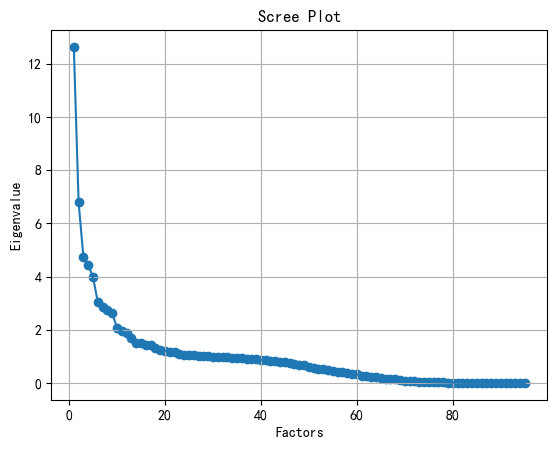
\includegraphics[width=.6\textwidth]{images/scree_plot.png}
    \caption{特征值大小变化作图,选择图中值突变位置对应的特征值个数}
    \label{fig:scree-plot}
\end{figure}
\par 为了能够更好的使用公共因子解释变量,希望每个变量仅在一个公因子上有较大的载荷,
使因子载荷矩阵中的元素值$a_{ij}^2$尽量靠近0或者1。为此,
选择方差最大旋转方法,寻找一个正交矩阵$\Gamma$对载荷矩阵$\Lambda$进行
旋转,得到$\tilde{\Lambda}=\Lambda\Gamma$。检查$\tilde{\Lambda}$
每一列元素平方的方差,期望方差最大。具体的,对于两个因子的载荷矩阵
$\Lambda = (a_{ij})_{p\times 2}$,取正交矩阵
\begin{equation*}
    \bm{T} =\left[
    \begin{array}{cc}
        \cos\phi & -\sin\phi \\
        \sin\phi & \cos\phi
    \end{array}
    \right]
\end{equation*}
将$\Lambda$旋转为$\tilde{\Lambda}=\Lambda T$,且$\tilde{\Lambda}$为参数
$\phi$的函数。对于$\tilde{\Lambda}$的列求平方,得到$b_{ij}=\tilde{a_{ij}}^2$,
最大化目标函数
\begin{equation*}
\max_{\phi} \ f(\phi)=Var(b_{11},b_{21},\ldots,b_{p1}) + Var(b_{12},b_{22},\ldots,b_{p2})
\end{equation*}
考虑$\nabla_{\phi}f(\phi)=0$,求解得到旋转参数$\phi$。对于$m$个变量,
需要进行$\binom{m}{2}$次旋转作为一个循环。完成后开始下一个循环,直到
方差收敛为止。旋转后得到的载荷矩阵$\Lambda$可视化如图\ref{fig:after-varimax-rotation}。
\begin{figure}[ht]
    \centering
    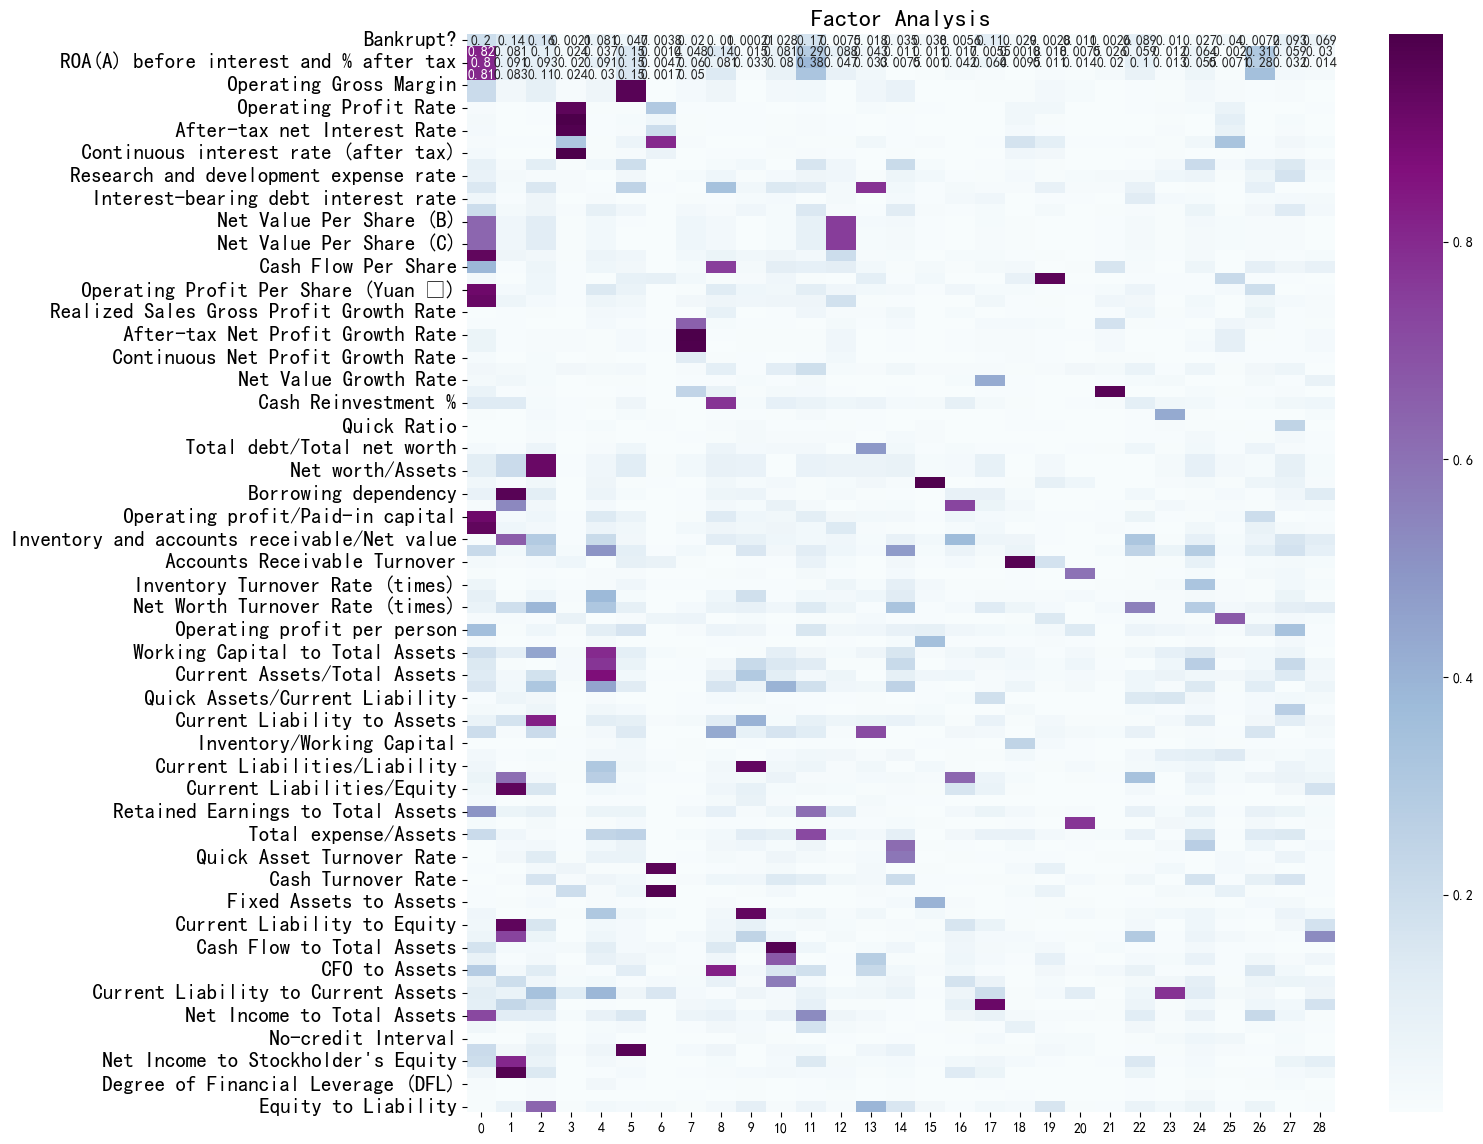
\includegraphics[width=.7\textwidth]{images/factor_analysis_varimax.png}
    \caption{载荷矩阵经历方差最大旋转后的热度图,其中每一个元素代表
    相应特征和因子的相关系数,颜色越深,因子与特征的关系越密切}
    \label{fig:after-varimax-rotation}
\end{figure}
可以观察到,经历方差最大旋转后,每一列中几乎只有一个深色的元素,代表
该因子与相应的特征关系密切,因子分析效果较好。但是由于本问题特征较多,
选择的因子数量也较多,所以对因子进行具体的解释较为繁琐,这里为了简化模型,
不对因子的含义进行具体解释。

\subsubsection{基于因子得分的公司经营情况排名}
因子的得分来源于原始样本对因子的测度,即把公共因子表示为原变量的线性组合:
\begin{equation}
F_{j}=c_j + \beta_{j1}X_1+\ldots+ \beta_{jp}X_p
\label{eq:score-for-one-factor}
\end{equation}
当求得其中的系数$(c_j,\beta_{j1},\ldots,\beta_{jp})$后,对于每个因子
$F_j$可以用式\ref{eq:score-mutual-information}求得因子得分,再
对每个因子得分进行线性加权得到最终的公司评分。
\par 由于特殊因子$\bm{\varepsilon}$的方差相异,
采用加权最小二乘法估计因子得分中的参数。即要使
\begin{equation*}
\nabla_{\bm{F}} (\bm{X-\mu-\Lambda F})^T \bm{\Psi}^{-1} (\bm{X-\mu-\Lambda F}) = 0
\end{equation*}
求解得到因子得分向量
\begin{equation*}
\hat{\bm{F}}=(\bm{\Lambda}^T\bm{\Psi}^{-1}\bm{\Lambda})^{-1}
\bm{\Lambda}^T \bm{\Psi}^{-1} (\bm{X}-\bm{\mu})
\end{equation*}
利用每个因子的方差贡献度对相应的因子得分进行加权,记方差贡献度向量为
$\bm{v}=(\lambda_1,\ldots,\lambda_m)$则公司$i$最终得分为
\begin{equation*}
S(i) = \bm{v}^T \hat{\bm{F}}
\end{equation*}
最终得到经营状况排名前10的公司记录在表\ref{tab:order-company}中。
\begin{table}[ht]
\centering
    \begin{tabular}{@{}lllllllllll@{}}
    \toprule[1.5pt]
    公司编号 & 5257  & 4023  & 2364  & 5609  & 2248  & 2055  & 4037  & 4185  & 2388  & 5808  \\ \midrule[0.5pt]
    公司得分 & 48.06 & 43.56 & 43.49 & 43.39 & 43.28 & 43.12 & 43.06 & 43.02 & 43.02 & 42.78 \\ \bottomrule[1.5pt]
    \end{tabular}
\caption{根据因子加权得分的公司经营情况排名(前10名)}
\label{tab:order-company}
\end{table}